\documentclass{article}
\usepackage[T1]{fontenc}
\usepackage{graphicx}
\usepackage{lipsum} % produce dummy text as filler
\usepackage{float}
\usepackage{trivfloat}
\trivfloat{image}
\usepackage{hyperref}
\graphicspath{{image/}}
\begin{document}
This picture
\begin{center}
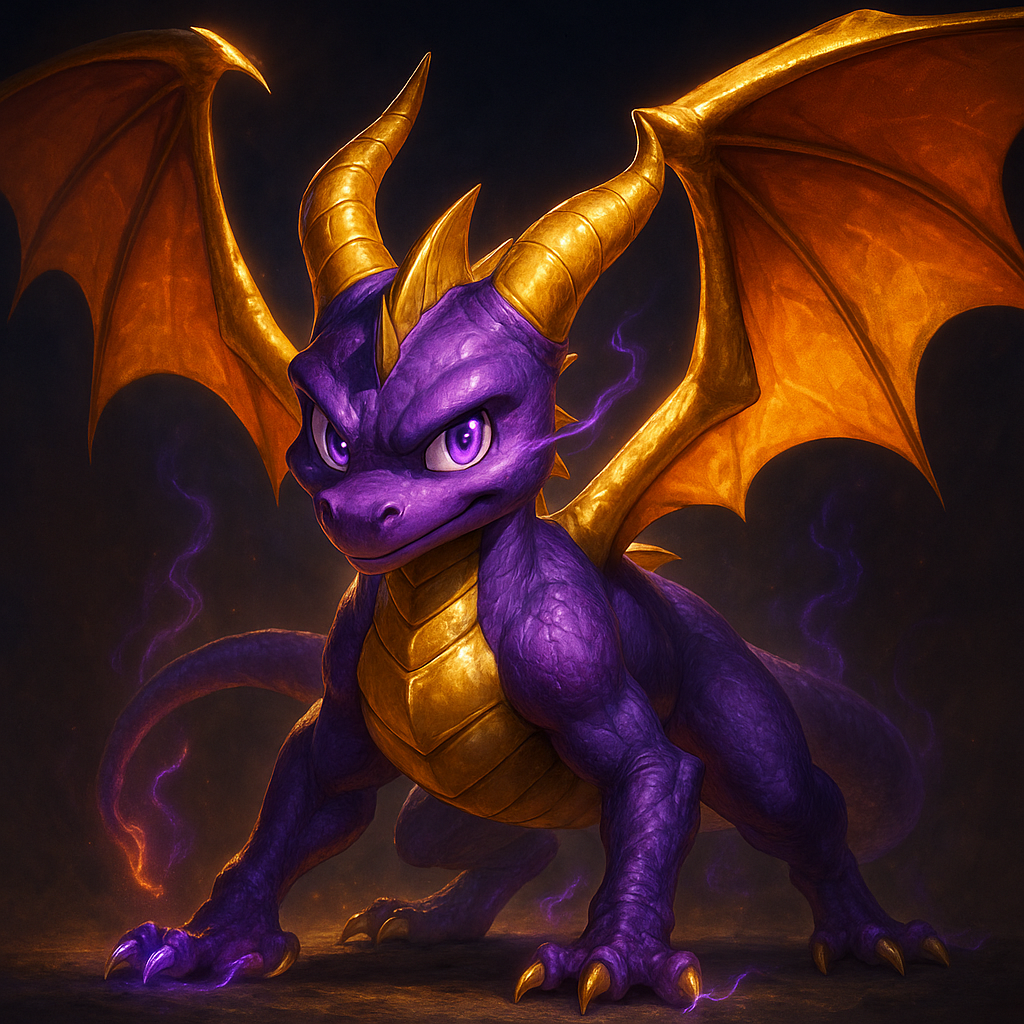
\includegraphics[height=2cm]{example-image.png}
\end{center}
is an imported PDF.



%-------------------------------

\begin{center}
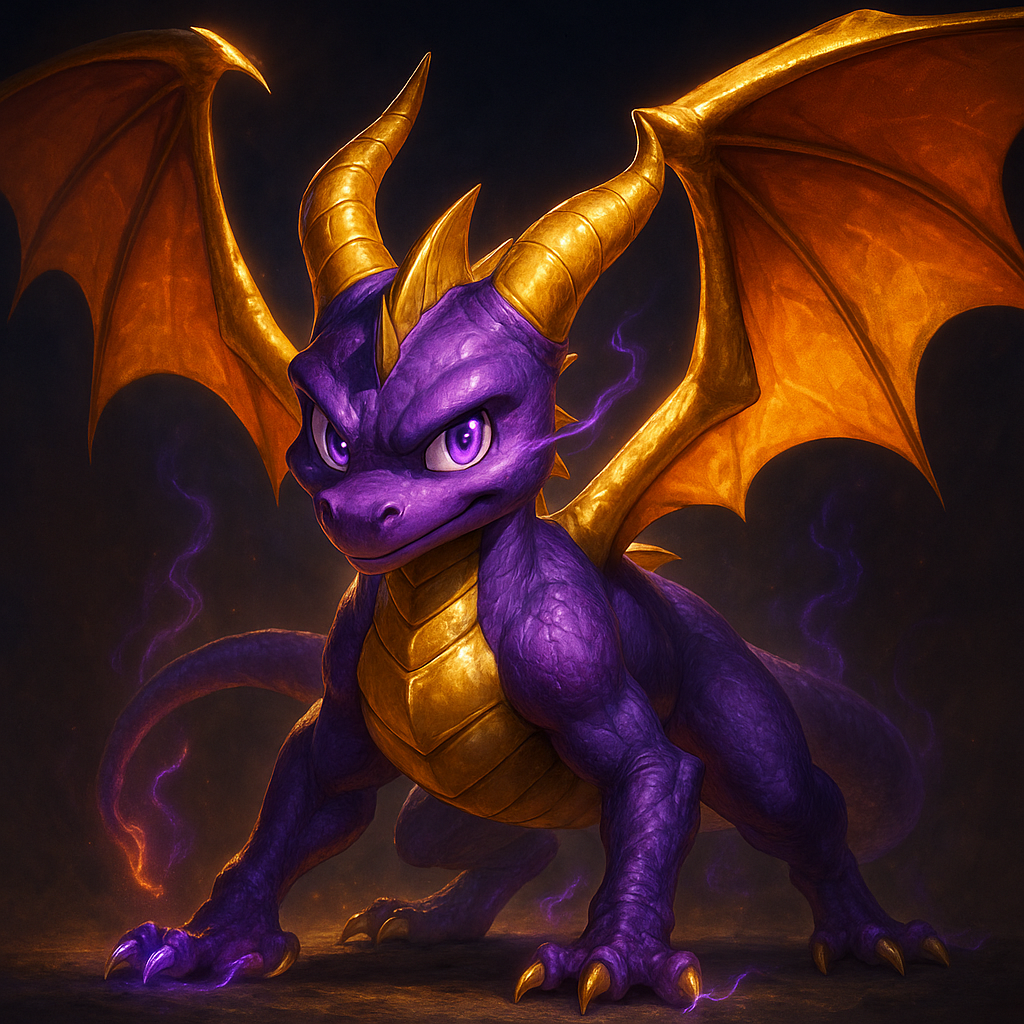
\includegraphics[height = 0.5\textheight]{example-image.png}
\end{center}
Some text
\begin{center}
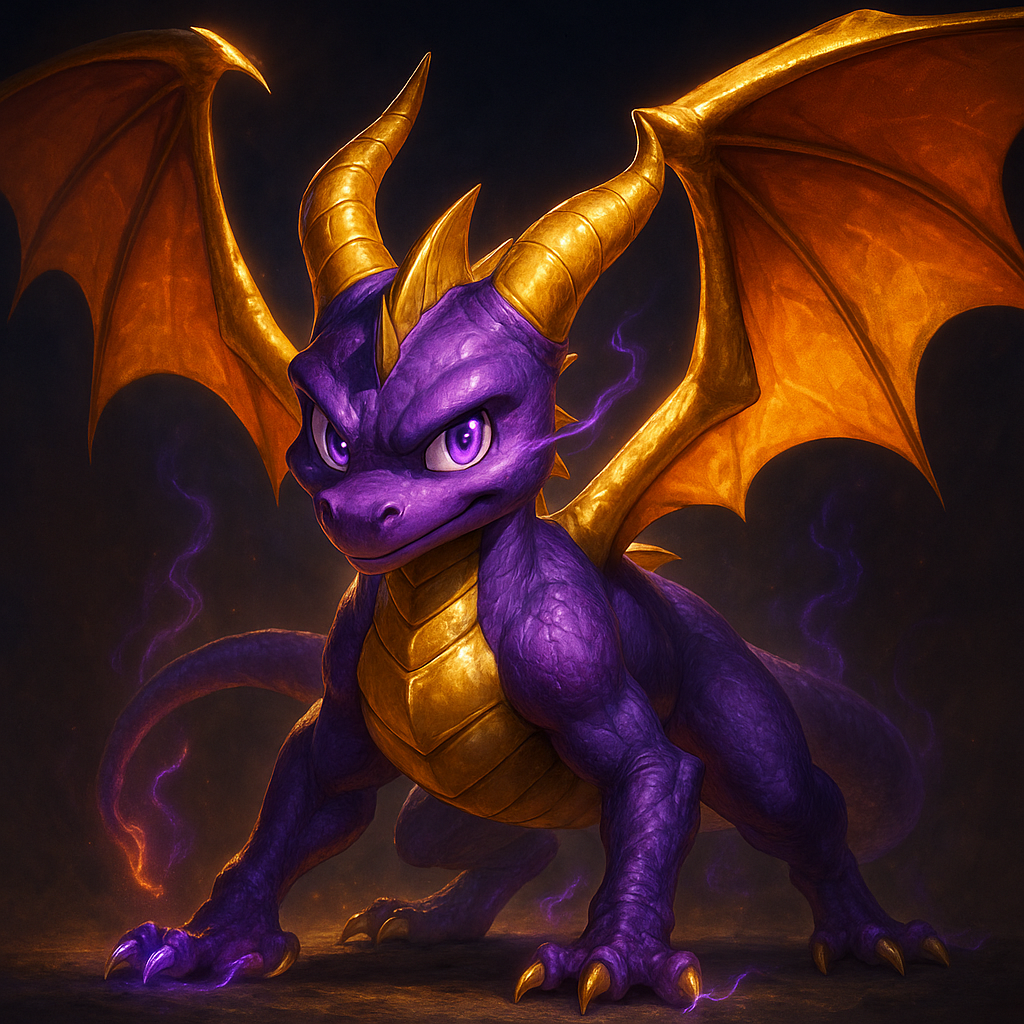
\includegraphics[width = 0.5\textwidth]{example-image.png}
\end{center}

\begin{center}
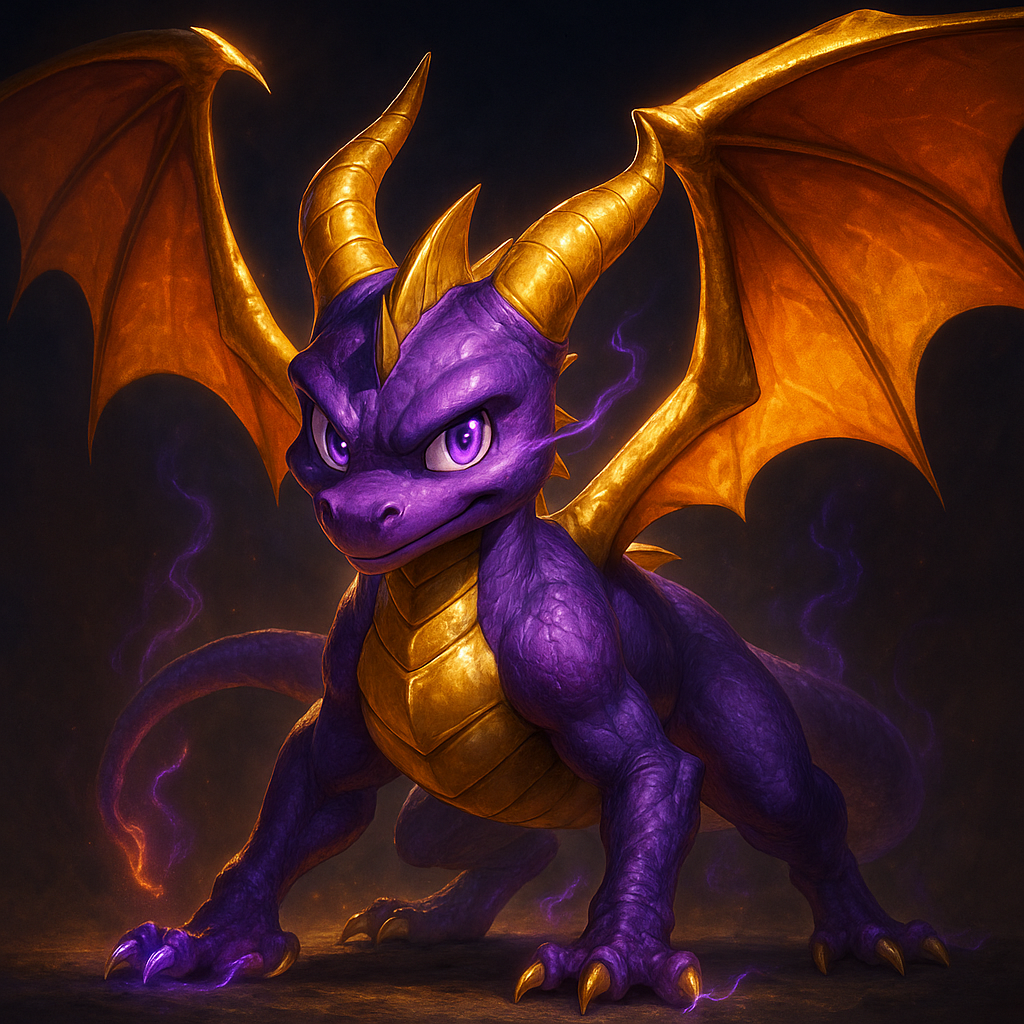
\includegraphics[clip, trim = 0 0 50 50]{example-image.png}
\end{center}

%------------------------

\lipsum[1-4] % Just a few filler paragraphs
Test location.
\begin{figure}[ht]
\centering
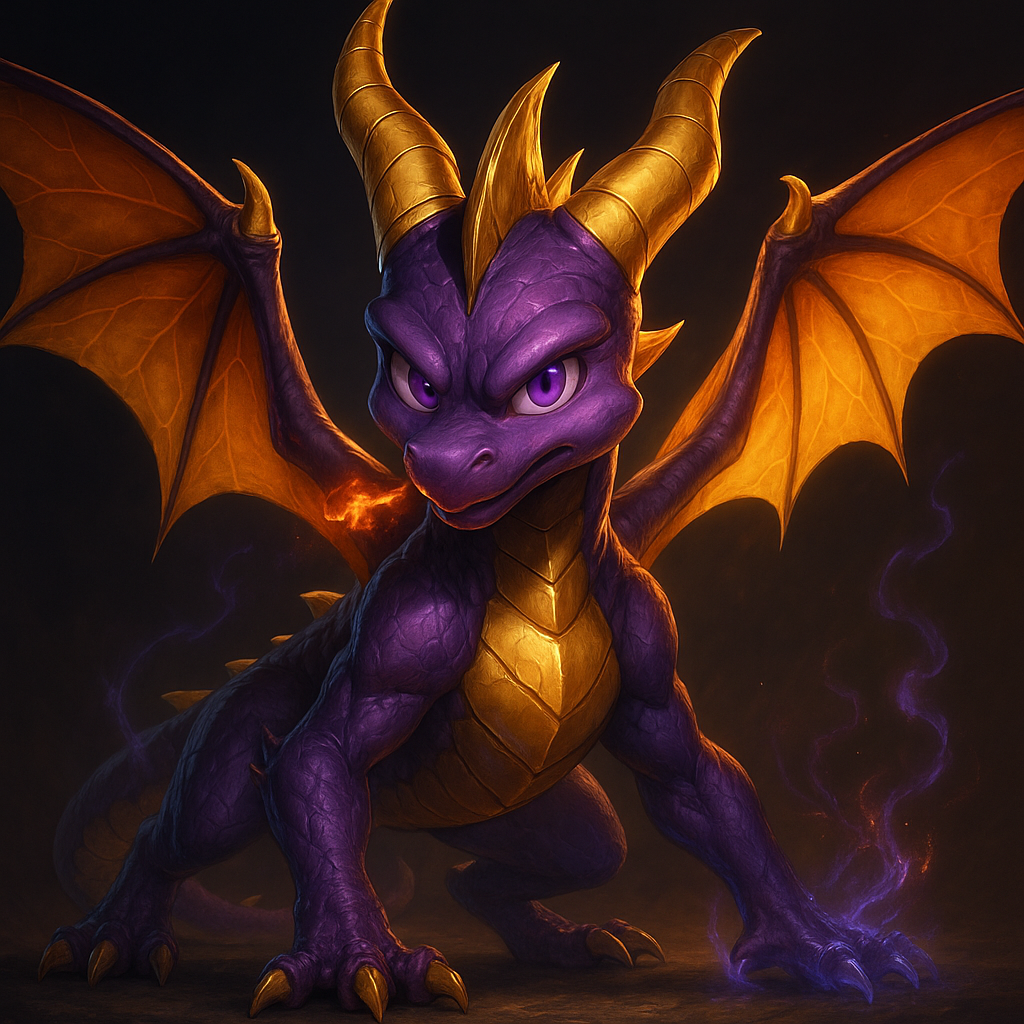
\includegraphics[width=0.5\textwidth]{example-image-a.png}
\caption{An example image}
\end{figure}
\lipsum[6-10] % Just a few filler paragraphs

%------------------------

An image from directory
\begin{figure}[ht]
\centering
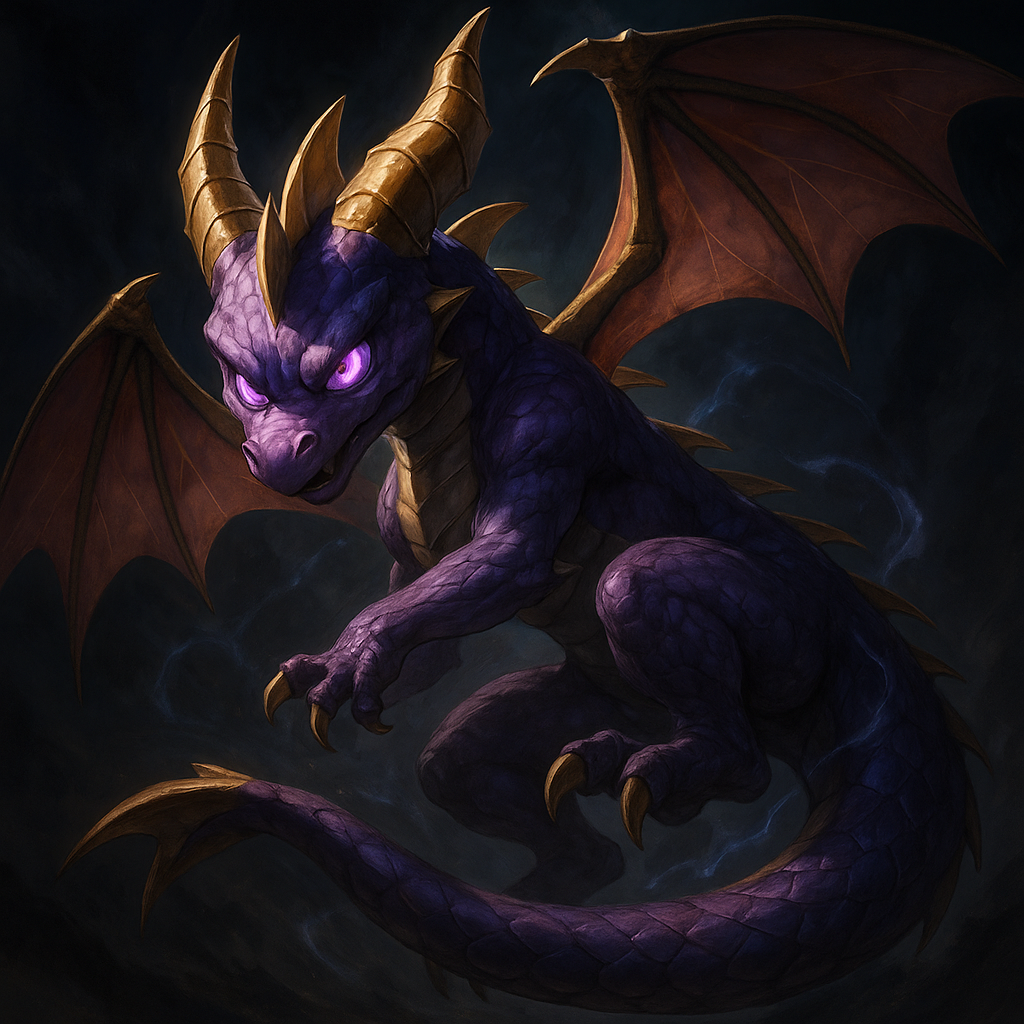
\includegraphics[width=0.5\textwidth]{example-image_b.png}
\caption{An example image from directory}
\end{figure}

%------------------------

\lipsum[1-8]
\begin{figure}[H]
\centering
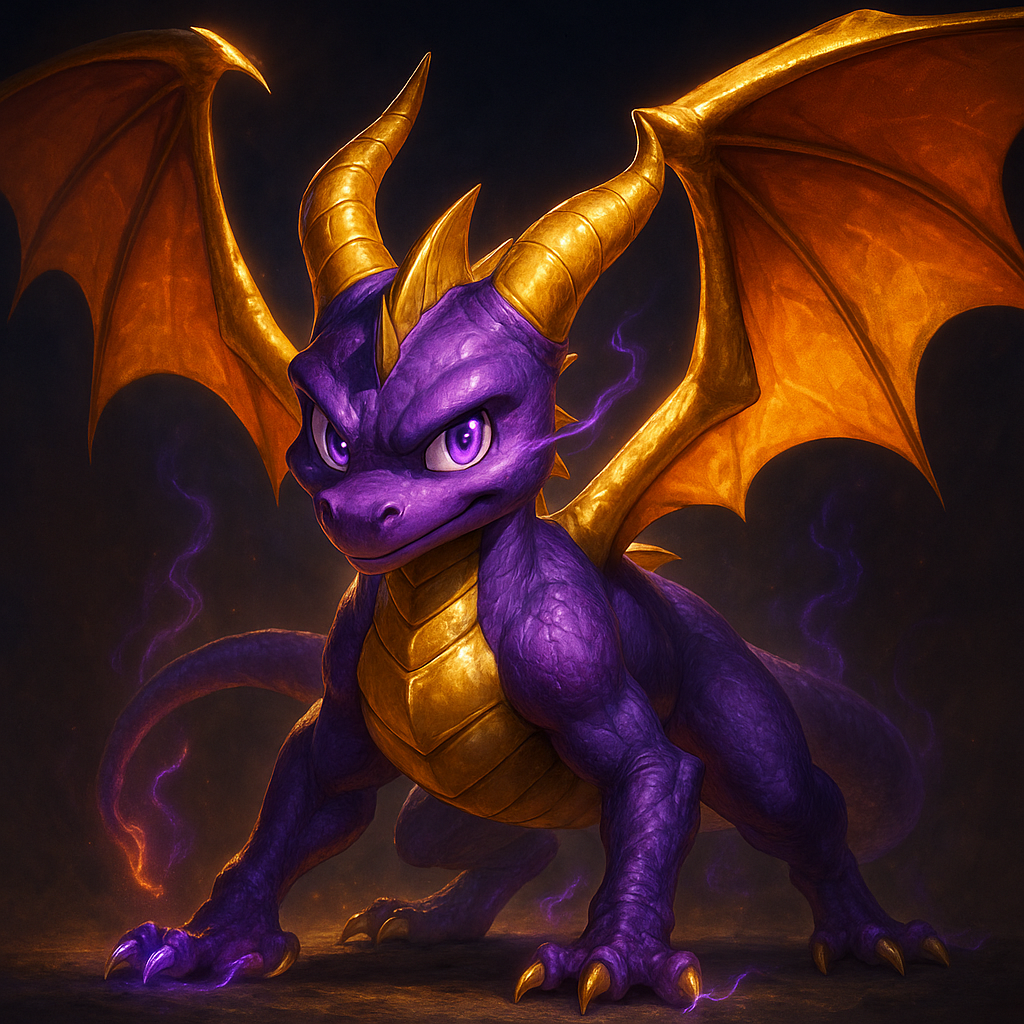
\includegraphics[width=0.5\textwidth]{example-image.png}
\caption{An example image}
\end{figure}
\lipsum[9-16]

%------------------------

trivfloat image
\begin{image}
\centering
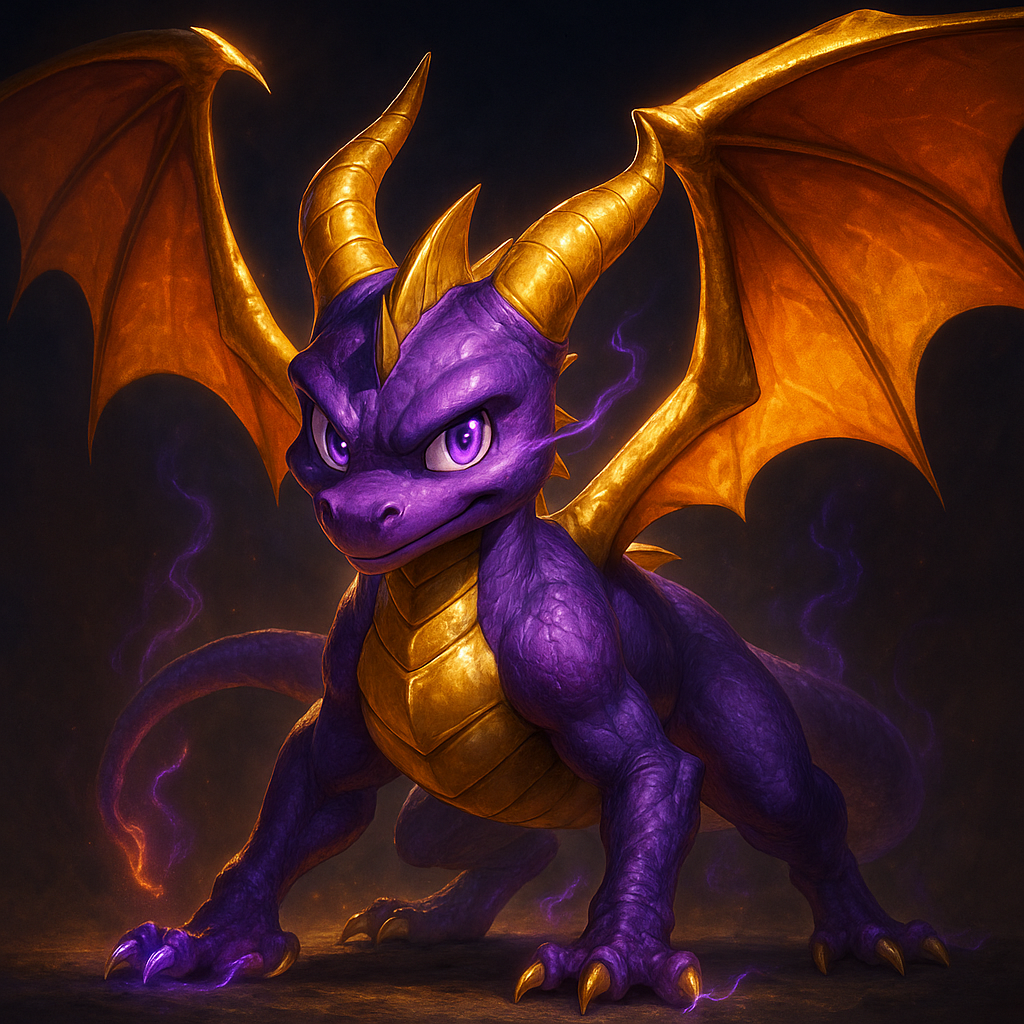
\includegraphics[width=0.5\textwidth]{example-image.png}
\caption{An example image}
\end{image}

%------------------------

Hey world!

This is a first document.

\section{Title of the first section}

Text of material for the first section.

\subsection{Subsection of the first section}
\label{subsec:labelone}

Text of material for the first subsection.
\begin{equation}
e^{i\pi}+1 = 0
\label{eq:labeltwo}
\end{equation}

In subsection~\ref{subsec:labelone} is equation~\ref{eq:labeltwo}.

%------------------------

\section{Introduction}

Some exciting text with a reference~\ref{sec:next}.

\section{Next thing}
\label{sec:next}

More text here. \lipsum[1]

%------------------------
%------------------------

Using different image options at Fig.~\ref{fig:my_image}.
\begin{figure}[H]
    \centering
    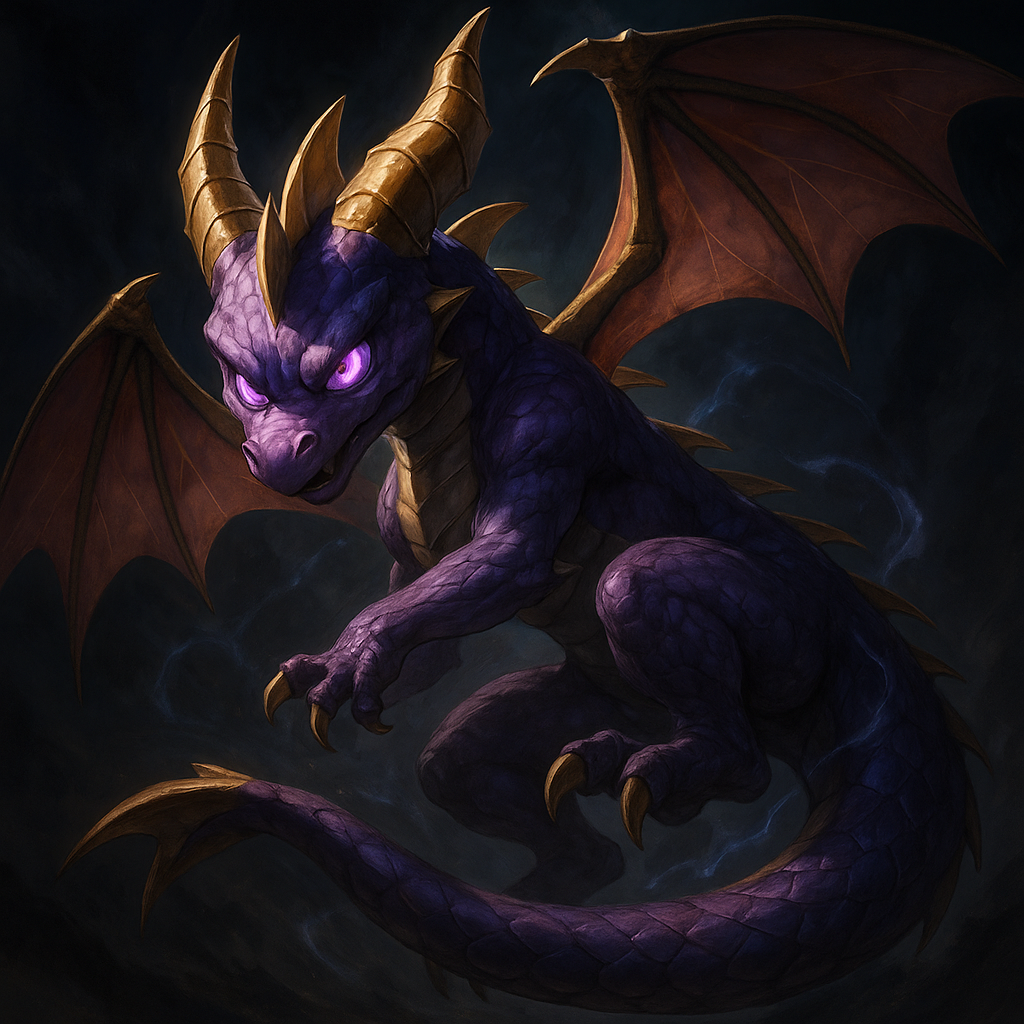
\includegraphics[width=0.7\textwidth,
                     height=4cm,
                     scale=0.8,
                     angle=15]
                     {example-image_b.png}
    \caption{Application of the options width, height, scale and angle}
    \label{fig:my_image}
\end{figure}

%------------------------

\lipsum[1-3]
\begin{figure}[!htbp]
\centering
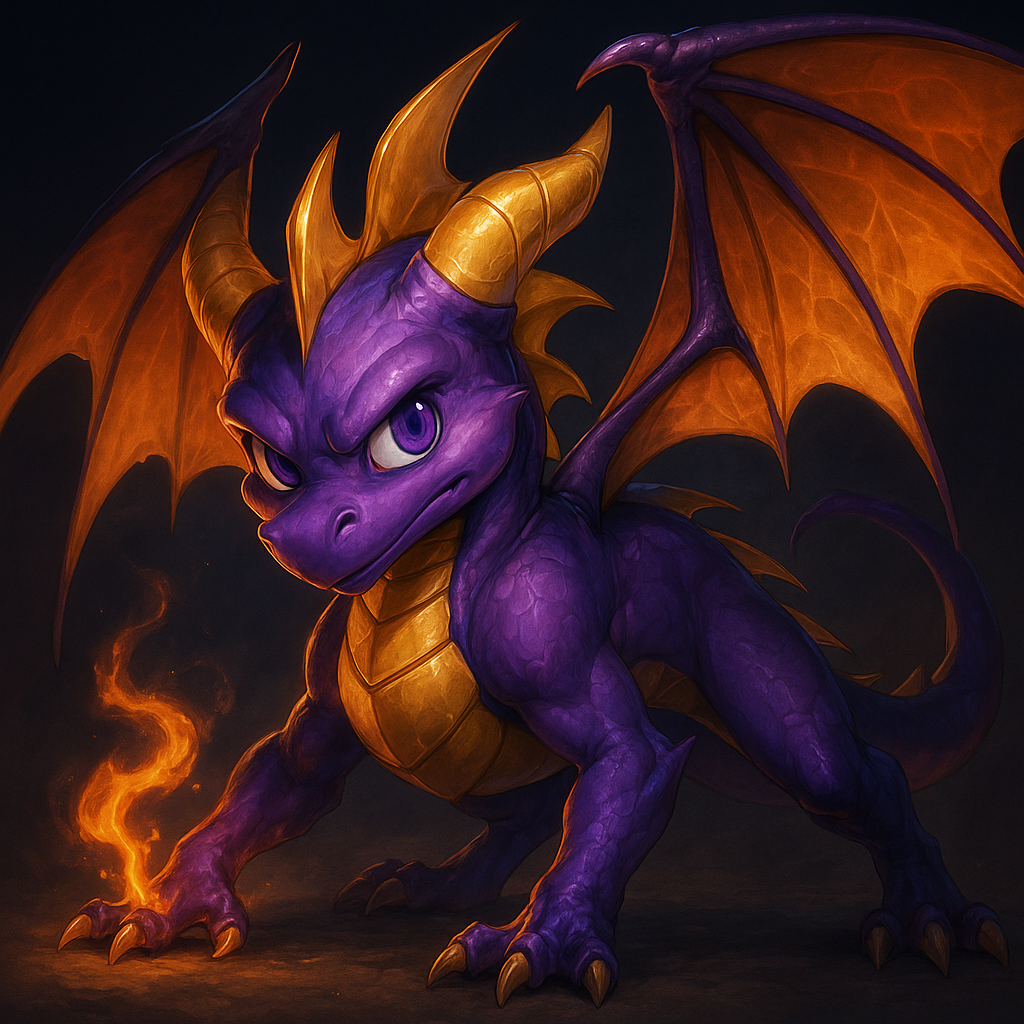
\includegraphics[width=0.5\textwidth]{example-image-c.png}
\caption{An example image}
\end{figure}
\lipsum[4-5]

%------------------------

\section{Label Test}
\label{sec:labtest}

Text of the section~\ref{sec:labtest} for label testing.

\subsection{Enumerate label test}
\label{subsec:enlabtest}

Here in subsection~\ref{subsec:enlabtest} we test enumerate list and it's label~\ref{en:test}
\begin{enumerate}
\label{en:test}
\item \lipsum[1]
\item \lipsum[2]
\end{enumerate}

Then we test wrong label to an image with a caption.
\begin{figure}[H]
    \centering
    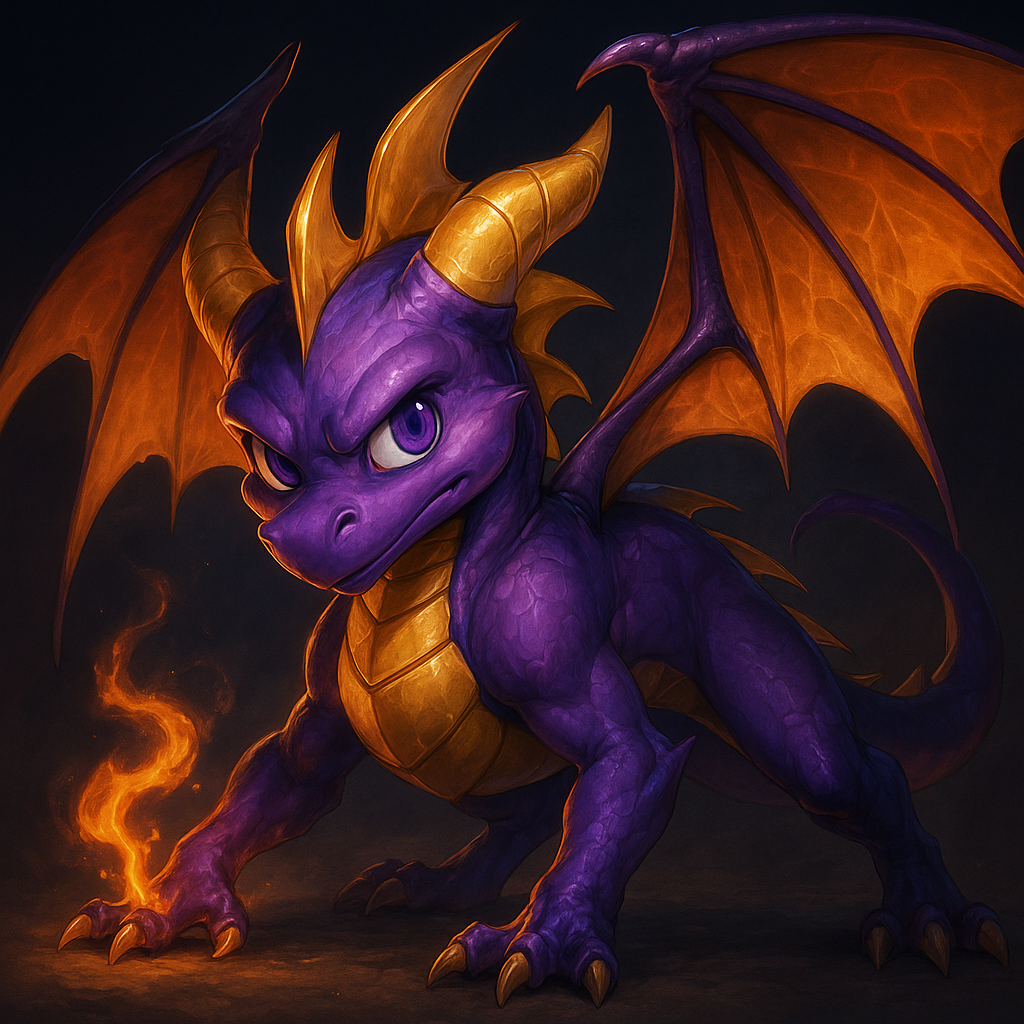
\includegraphics[width=0.3\textwidth]{example-image-c.png}
    \label{fig:wrong_label_order} % Неправильно!
    \caption{A figure with incorrect label order.}
\end{figure}
A reference to figure~\ref{fig:wrong_label_order}. % Ссылка будет на номер подраздела

\subsection{Equation label test}
\label{subsec:eqlabtest}

And finally, here in subsection~\ref{subsec:eqlabtest} we test wrong label for an equation~\ref{eq:test}
\begin{equation}
e = mc^2
\end{equation}
\label{eq:test} 

\end{document}